\documentclass[1p]{elsarticle_modified}
%\bibliographystyle{elsarticle-num}

%\usepackage[colorlinks]{hyperref}
%\usepackage{abbrmath_seonhwa} %\Abb, \Ascr, \Acal ,\Abf, \Afrak
\usepackage{amsfonts}
\usepackage{amssymb}
\usepackage{amsmath}
\usepackage{amsthm}
\usepackage{scalefnt}
\usepackage{amsbsy}
\usepackage{kotex}
\usepackage{caption}
\usepackage{subfig}
\usepackage{color}
\usepackage{graphicx}
\usepackage{xcolor} %% white, black, red, green, blue, cyan, magenta, yellow
\usepackage{float}
\usepackage{setspace}
\usepackage{hyperref}

\usepackage{tikz}
\usetikzlibrary{arrows}

\usepackage{multirow}
\usepackage{array} % fixed length table
\usepackage{hhline}

%%%%%%%%%%%%%%%%%%%%%
\makeatletter
\renewcommand*\env@matrix[1][\arraystretch]{%
	\edef\arraystretch{#1}%
	\hskip -\arraycolsep
	\let\@ifnextchar\new@ifnextchar
	\array{*\c@MaxMatrixCols c}}
\makeatother %https://tex.stackexchange.com/questions/14071/how-can-i-increase-the-line-spacing-in-a-matrix
%%%%%%%%%%%%%%%

\usepackage[normalem]{ulem}

\newcommand{\msout}[1]{\ifmmode\text{\sout{\ensuremath{#1}}}\else\sout{#1}\fi}
%SOURCE: \msout is \stkout macro in https://tex.stackexchange.com/questions/20609/strikeout-in-math-mode

\newcommand{\cancel}[1]{
	\ifmmode
	{\color{red}\msout{#1}}
	\else
	{\color{red}\sout{#1}}
	\fi
}

\newcommand{\add}[1]{
	{\color{blue}\uwave{#1}}
}

\newcommand{\replace}[2]{
	\ifmmode
	{\color{red}\msout{#1}}{\color{blue}\uwave{#2}}
	\else
	{\color{red}\sout{#1}}{\color{blue}\uwave{#2}}
	\fi
}

\newcommand{\Sol}{\mathcal{S}} %segment
\newcommand{\D}{D} %diagram
\newcommand{\A}{\mathcal{A}} %arc


%%%%%%%%%%%%%%%%%%%%%%%%%%%%%5 test

\def\sl{\operatorname{\textup{SL}}(2,\Cbb)}
\def\psl{\operatorname{\textup{PSL}}(2,\Cbb)}
\def\quan{\mkern 1mu \triangleright \mkern 1mu}

\theoremstyle{definition}
\newtheorem{thm}{Theorem}[section]
\newtheorem{prop}[thm]{Proposition}
\newtheorem{lem}[thm]{Lemma}
\newtheorem{ques}[thm]{Question}
\newtheorem{cor}[thm]{Corollary}
\newtheorem{defn}[thm]{Definition}
\newtheorem{exam}[thm]{Example}
\newtheorem{rmk}[thm]{Remark}
\newtheorem{alg}[thm]{Algorithm}

\newcommand{\I}{\sqrt{-1}}
\begin{document}

%\begin{frontmatter}
%
%\title{Boundary parabolic representations of knots up to 8 crossings}
%
%%% Group authors per affiliation:
%\author{Yunhi Cho} 
%\address{Department of Mathematics, University of Seoul, Seoul, Korea}
%\ead{yhcho@uos.ac.kr}
%
%
%\author{Seonhwa Kim} %\fnref{s_kim}}
%\address{Center for Geometry and Physics, Institute for Basic Science, Pohang, 37673, Korea}
%\ead{ryeona17@ibs.re.kr}
%
%\author{Hyuk Kim}
%\address{Department of Mathematical Sciences, Seoul National University, Seoul 08826, Korea}
%\ead{hyukkim@snu.ac.kr}
%
%\author{Seokbeom Yoon}
%\address{Department of Mathematical Sciences, Seoul National University, Seoul, 08826,  Korea}
%\ead{sbyoon15@snu.ac.kr}
%
%\begin{abstract}
%We find all boundary parabolic representation of knots up to 8 crossings.
%
%\end{abstract}
%\begin{keyword}
%    \MSC[2010] 57M25 
%\end{keyword}
%
%\end{frontmatter}

%\linenumbers
%\tableofcontents
%
\newcommand\colored[1]{\textcolor{white}{\rule[-0.35ex]{0.8em}{1.4ex}}\kern-0.8em\color{red} #1}%
%\newcommand\colored[1]{\textcolor{white}{ #1}\kern-2.17ex	\textcolor{white}{ #1}\kern-1.81ex	\textcolor{white}{ #1}\kern-2.15ex\color{red}#1	}

{\Large $\underline{12a_{0659}~(K12a_{0659})}$}

\setlength{\tabcolsep}{10pt}
\renewcommand{\arraystretch}{1.6}
\vspace{1cm}\begin{tabular}{m{100pt}>{\centering\arraybackslash}m{274pt}}
\multirow{5}{120pt}{
	\centering
	\includegraphics[width=112pt]{../../../GIT/diagram.site/Diagrams/png/1460_12a_0659.png}\\
\ \ \ A knot diagram\footnotemark}&
\allowdisplaybreaks
\textbf{Linearized knot diagam} \\
\cline{2-2}
 &
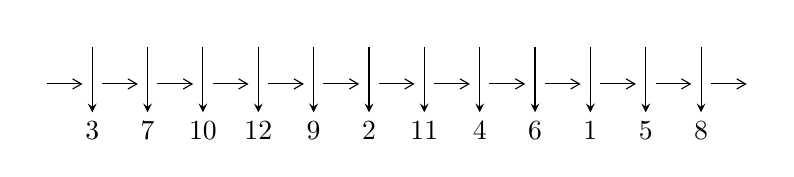
\begin{tikzpicture}[x=20pt, y=17pt]
	% nodes
	\node (C0) at (0, 0) {};
	\node (C1) at (1, 0) {};
	\node (C1U) at (1, +1) {};
	\node (C1D) at (1, -1) {3};

	\node (C2) at (2, 0) {};
	\node (C2U) at (2, +1) {};
	\node (C2D) at (2, -1) {7};

	\node (C3) at (3, 0) {};
	\node (C3U) at (3, +1) {};
	\node (C3D) at (3, -1) {10};

	\node (C4) at (4, 0) {};
	\node (C4U) at (4, +1) {};
	\node (C4D) at (4, -1) {12};

	\node (C5) at (5, 0) {};
	\node (C5U) at (5, +1) {};
	\node (C5D) at (5, -1) {9};

	\node (C6) at (6, 0) {};
	\node (C6U) at (6, +1) {};
	\node (C6D) at (6, -1) {2};

	\node (C7) at (7, 0) {};
	\node (C7U) at (7, +1) {};
	\node (C7D) at (7, -1) {11};

	\node (C8) at (8, 0) {};
	\node (C8U) at (8, +1) {};
	\node (C8D) at (8, -1) {4};

	\node (C9) at (9, 0) {};
	\node (C9U) at (9, +1) {};
	\node (C9D) at (9, -1) {6};

	\node (C10) at (10, 0) {};
	\node (C10U) at (10, +1) {};
	\node (C10D) at (10, -1) {1};

	\node (C11) at (11, 0) {};
	\node (C11U) at (11, +1) {};
	\node (C11D) at (11, -1) {5};

	\node (C12) at (12, 0) {};
	\node (C12U) at (12, +1) {};
	\node (C12D) at (12, -1) {8};
	\node (C13) at (13, 0) {};

	% arrows
	\draw[->,>={angle 60}]
	(C0) edge (C1) (C1) edge (C2) (C2) edge (C3) (C3) edge (C4) (C4) edge (C5) (C5) edge (C6) (C6) edge (C7) (C7) edge (C8) (C8) edge (C9) (C9) edge (C10) (C10) edge (C11) (C11) edge (C12) (C12) edge (C13) ;	\draw[->,>=stealth]
	(C1U) edge (C1D) (C2U) edge (C2D) (C3U) edge (C3D) (C4U) edge (C4D) (C5U) edge (C5D) (C6U) edge (C6D) (C7U) edge (C7D) (C8U) edge (C8D) (C9U) edge (C9D) (C10U) edge (C10D) (C11U) edge (C11D) (C12U) edge (C12D) ;
	\end{tikzpicture} \\
\hhline{~~} \\& 
\textbf{Solving Sequence} \\ \cline{2-2} 
 &
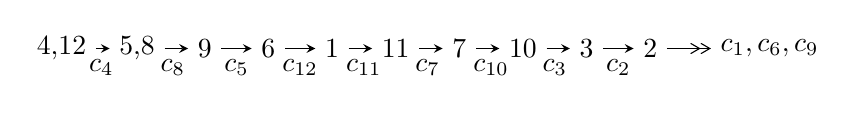
\begin{tikzpicture}[x=23pt, y=7pt]
	% node
	\node (A0) at (-1/8, 0) {4,12};
	\node (A1) at (17/16, 0) {5,8};
	\node (A2) at (17/8, 0) {9};
	\node (A3) at (25/8, 0) {6};
	\node (A4) at (33/8, 0) {1};
	\node (A5) at (41/8, 0) {11};
	\node (A6) at (49/8, 0) {7};
	\node (A7) at (57/8, 0) {10};
	\node (A8) at (65/8, 0) {3};
	\node (A9) at (73/8, 0) {2};
	\node (C1) at (1/2, -1) {$c_{4}$};
	\node (C2) at (13/8, -1) {$c_{8}$};
	\node (C3) at (21/8, -1) {$c_{5}$};
	\node (C4) at (29/8, -1) {$c_{12}$};
	\node (C5) at (37/8, -1) {$c_{11}$};
	\node (C6) at (45/8, -1) {$c_{7}$};
	\node (C7) at (53/8, -1) {$c_{10}$};
	\node (C8) at (61/8, -1) {$c_{3}$};
	\node (C9) at (69/8, -1) {$c_{2}$};
	\node (A10) at (11, 0) {$c_{1},c_{6},c_{9}$};

	% edge
	\draw[->,>=stealth]	
	(A0) edge (A1) (A1) edge (A2) (A2) edge (A3) (A3) edge (A4) (A4) edge (A5) (A5) edge (A6) (A6) edge (A7) (A7) edge (A8) (A8) edge (A9) ;
	\draw[->>,>={angle 60}]	
	(A9) edge (A10);
\end{tikzpicture} \\ 

\end{tabular} \\

\footnotetext{
The image of knot diagram is generated by the software ``\textbf{Draw programme}" developed by Andrew Bartholomew(\url{http://www.layer8.co.uk/maths/draw/index.htm\#Running-draw}), where we modified some parts for our purpose(\url{https://github.com/CATsTAILs/LinksPainter}).
}\phantom \\ \newline 
\centering \textbf{Ideals for irreducible components\footnotemark of $X_{\text{par}}$} 
 
\begin{align*}
I^u_{1}&=\langle 
3.09510\times10^{887} u^{168}+1.93391\times10^{887} u^{167}+\cdots+5.11630\times10^{888} b-1.15540\times10^{892},\\
\phantom{I^u_{1}}&\phantom{= \langle  }7.90794\times10^{888} u^{168}+1.64481\times10^{891} u^{167}+\cdots+9.53897\times10^{891} a+2.08425\times10^{895},\\
\phantom{I^u_{1}}&\phantom{= \langle  }u^{169}+2 u^{168}+\cdots+65269 u+13051\rangle \\
I^u_{2}&=\langle 
-9.26459\times10^{33} u^{37}+1.06188\times10^{34} u^{36}+\cdots+3.68110\times10^{33} b-4.69466\times10^{34},\\
\phantom{I^u_{2}}&\phantom{= \langle  }1.86555\times10^{34} u^{37}+2.19102\times10^{34} u^{36}+\cdots+2.57677\times10^{34} a-3.37189\times10^{35},\;u^{38}- u^{37}+\cdots+3 u-7\rangle \\
\\
\end{align*}
\raggedright * 2 irreducible components of $\dim_{\mathbb{C}}=0$, with total 207 representations.\\
\footnotetext{All coefficients of polynomials are rational numbers. But the coefficients are sometimes approximated in decimal forms when there is not enough margin.}
\newpage
\renewcommand{\arraystretch}{1}
\centering \section*{I. $I^u_{1}= \langle 3.10\times10^{887} u^{168}+1.93\times10^{887} u^{167}+\cdots+5.12\times10^{888} b-1.16\times10^{892},\;7.91\times10^{888} u^{168}+1.64\times10^{891} u^{167}+\cdots+9.54\times10^{891} a+2.08\times10^{895},\;u^{169}+2 u^{168}+\cdots+65269 u+13051 \rangle$}
\flushleft \textbf{(i) Arc colorings}\\
\begin{tabular}{m{7pt} m{180pt} m{7pt} m{180pt} }
\flushright $a_{4}=$&$\begin{pmatrix}1\\0\end{pmatrix}$ \\
\flushright $a_{12}=$&$\begin{pmatrix}0\\u\end{pmatrix}$ \\
\flushright $a_{5}=$&$\begin{pmatrix}1\\u^2\end{pmatrix}$ \\
\flushright $a_{8}=$&$\begin{pmatrix}-0.000829014 u^{168}-0.172431 u^{167}+\cdots-12895.8 u-2184.99\\-0.0604950 u^{168}-0.0377989 u^{167}+\cdots+12402.5 u+2258.27\end{pmatrix}$ \\
\flushright $a_{9}=$&$\begin{pmatrix}0.0596660 u^{168}-0.134632 u^{167}+\cdots-25298.3 u-4443.26\\-0.0604950 u^{168}-0.0377989 u^{167}+\cdots+12402.5 u+2258.27\end{pmatrix}$ \\
\flushright $a_{6}=$&$\begin{pmatrix}0.349624 u^{168}+0.751468 u^{167}+\cdots-2742.15 u-1350.08\\-0.295949 u^{168}-0.736332 u^{167}+\cdots-3667.78 u+102.662\end{pmatrix}$ \\
\flushright $a_{1}=$&$\begin{pmatrix}0.0470350 u^{168}+0.0467437 u^{167}+\cdots-7824.49 u-1349.44\\-0.105932 u^{168}-0.194999 u^{167}+\cdots+6946.06 u+1538.27\end{pmatrix}$ \\
\flushright $a_{11}=$&$\begin{pmatrix}u\\u^3+u\end{pmatrix}$ \\
\flushright $a_{7}=$&$\begin{pmatrix}0.0906963 u^{168}-0.0344680 u^{167}+\cdots-22511.8 u-3998.89\\-0.100914 u^{168}-0.208313 u^{167}+\cdots+4534.85 u+1032.82\end{pmatrix}$ \\
\flushright $a_{10}=$&$\begin{pmatrix}-0.447630 u^{168}-0.986075 u^{167}+\cdots-2487.51 u+557.448\\0.149530 u^{168}+0.381710 u^{167}+\cdots+2813.98 u+79.8128\end{pmatrix}$ \\
\flushright $a_{3}=$&$\begin{pmatrix}0.158314 u^{168}+0.624237 u^{167}+\cdots+19953.4 u+3201.62\\0.00889723 u^{168}-0.170628 u^{167}+\cdots-17746.0 u-3123.31\end{pmatrix}$ \\
\flushright $a_{2}=$&$\begin{pmatrix}-0.00970490 u^{168}+0.419594 u^{167}+\cdots+39719.3 u+7112.40\\0.0498702 u^{168}-0.124749 u^{167}+\cdots-21725.9 u-4006.80\end{pmatrix}$\\&\end{tabular}
\flushleft \textbf{(ii) Obstruction class $= -1$}\\~\\
\flushleft \textbf{(iii) Cusp Shapes $= -1.41920 u^{168}-2.44682 u^{167}+\cdots+38884.9 u+9544.51$}\\~\\
\newpage\renewcommand{\arraystretch}{1}
\flushleft \textbf{(iv) u-Polynomials at the component}\newline \\
\begin{tabular}{m{50pt}|m{274pt}}
Crossings & \hspace{64pt}u-Polynomials at each crossing \\
\hline $$\begin{aligned}c_{1}\end{aligned}$$&$\begin{aligned}
&u^{169}+80 u^{168}+\cdots+99813 u+2401
\end{aligned}$\\
\hline $$\begin{aligned}c_{2},c_{6}\end{aligned}$$&$\begin{aligned}
&u^{169}-2 u^{168}+\cdots-49 u+49
\end{aligned}$\\
\hline $$\begin{aligned}c_{3}\end{aligned}$$&$\begin{aligned}
&u^{169}+2 u^{168}+\cdots+11167 u+523
\end{aligned}$\\
\hline $$\begin{aligned}c_{4},c_{11}\end{aligned}$$&$\begin{aligned}
&u^{169}+2 u^{168}+\cdots+65269 u+13051
\end{aligned}$\\
\hline $$\begin{aligned}c_{5},c_{9}\end{aligned}$$&$\begin{aligned}
&u^{169}+16 u^{168}+\cdots+3871835 u+205027
\end{aligned}$\\
\hline $$\begin{aligned}c_{7}\end{aligned}$$&$\begin{aligned}
&u^{169}+4 u^{168}+\cdots-7867 u+18377
\end{aligned}$\\
\hline $$\begin{aligned}c_{8}\end{aligned}$$&$\begin{aligned}
&u^{169}- u^{168}+\cdots+2292504 u+164545
\end{aligned}$\\
\hline $$\begin{aligned}c_{10}\end{aligned}$$&$\begin{aligned}
&u^{169}-14 u^{168}+\cdots-13650 u+6089
\end{aligned}$\\
\hline $$\begin{aligned}c_{12}\end{aligned}$$&$\begin{aligned}
&u^{169}-3 u^{168}+\cdots+496671 u+144999
\end{aligned}$\\
\hline
\end{tabular}\\~\\
\newpage\renewcommand{\arraystretch}{1}
\flushleft \textbf{(v) Riley Polynomials at the component}\newline \\
\begin{tabular}{m{50pt}|m{274pt}}
Crossings & \hspace{64pt}Riley Polynomials at each crossing \\
\hline $$\begin{aligned}c_{1}\end{aligned}$$&$\begin{aligned}
&y^{169}+28 y^{168}+\cdots-55412679 y-5764801
\end{aligned}$\\
\hline $$\begin{aligned}c_{2},c_{6}\end{aligned}$$&$\begin{aligned}
&y^{169}-80 y^{168}+\cdots+99813 y-2401
\end{aligned}$\\
\hline $$\begin{aligned}c_{3}\end{aligned}$$&$\begin{aligned}
&y^{169}-14 y^{168}+\cdots-3774107 y-273529
\end{aligned}$\\
\hline $$\begin{aligned}c_{4},c_{11}\end{aligned}$$&$\begin{aligned}
&y^{169}+90 y^{168}+\cdots+67826243 y-170328601
\end{aligned}$\\
\hline $$\begin{aligned}c_{5},c_{9}\end{aligned}$$&$\begin{aligned}
&y^{169}-216 y^{168}+\cdots+4325021500815 y-42036070729
\end{aligned}$\\
\hline $$\begin{aligned}c_{7}\end{aligned}$$&$\begin{aligned}
&y^{169}+10 y^{168}+\cdots+44572417095 y-337714129
\end{aligned}$\\
\hline $$\begin{aligned}c_{8}\end{aligned}$$&$\begin{aligned}
&y^{169}+7 y^{168}+\cdots+2188189227116 y-27075057025
\end{aligned}$\\
\hline $$\begin{aligned}c_{10}\end{aligned}$$&$\begin{aligned}
&y^{169}+122 y^{168}+\cdots+1911336200 y-37075921
\end{aligned}$\\
\hline $$\begin{aligned}c_{12}\end{aligned}$$&$\begin{aligned}
&y^{169}+141 y^{168}+\cdots-1184216769423 y-21024710001
\end{aligned}$\\
\hline
\end{tabular}\\~\\
\newpage\flushleft \textbf{(vi) Complex Volumes and Cusp Shapes}
$$\begin{array}{c|c|c}  
\text{Solutions to }I^u_{1}& \I (\text{vol} + \sqrt{-1}CS) & \text{Cusp shape}\\
 \hline 
\begin{aligned}
u &= \phantom{-}0.071971 + 0.993217 I \\
a &= -6.75716 - 0.40615 I \\
b &= -0.147600 + 0.008410 I\end{aligned}
 & \phantom{-}0.07454 - 2.04421 I & \phantom{-0.000000 } 0 \\ \hline\begin{aligned}
u &= \phantom{-}0.071971 - 0.993217 I \\
a &= -6.75716 + 0.40615 I \\
b &= -0.147600 - 0.008410 I\end{aligned}
 & \phantom{-}0.07454 + 2.04421 I & \phantom{-0.000000 } 0 \\ \hline\begin{aligned}
u &= \phantom{-}0.404057 + 0.920241 I \\
a &= -0.21246 + 1.73079 I \\
b &= -1.079020 - 0.354825 I\end{aligned}
 & -6.35368 - 2.60436 I & \phantom{-0.000000 } 0 \\ \hline\begin{aligned}
u &= \phantom{-}0.404057 - 0.920241 I \\
a &= -0.21246 - 1.73079 I \\
b &= -1.079020 + 0.354825 I\end{aligned}
 & -6.35368 + 2.60436 I & \phantom{-0.000000 } 0 \\ \hline\begin{aligned}
u &= -0.824347 + 0.531630 I \\
a &= -0.013021 + 0.212634 I \\
b &= \phantom{-}0.737459 + 0.612624 I\end{aligned}
 & -5.27801 - 0.92055 I & \phantom{-0.000000 } 0 \\ \hline\begin{aligned}
u &= -0.824347 - 0.531630 I \\
a &= -0.013021 - 0.212634 I \\
b &= \phantom{-}0.737459 - 0.612624 I\end{aligned}
 & -5.27801 + 0.92055 I & \phantom{-0.000000 } 0 \\ \hline\begin{aligned}
u &= \phantom{-}0.390660 + 0.895610 I \\
a &= -1.053550 + 0.037286 I \\
b &= -0.23714 - 1.41292 I\end{aligned}
 & \phantom{-}4.19117 - 1.87219 I & \phantom{-0.000000 } 0 \\ \hline\begin{aligned}
u &= \phantom{-}0.390660 - 0.895610 I \\
a &= -1.053550 - 0.037286 I \\
b &= -0.23714 + 1.41292 I\end{aligned}
 & \phantom{-}4.19117 + 1.87219 I & \phantom{-0.000000 } 0 \\ \hline\begin{aligned}
u &= -0.188896 + 0.952600 I \\
a &= \phantom{-}1.54752 - 0.79819 I \\
b &= \phantom{-}0.576613 + 0.697087 I\end{aligned}
 & -0.96768 + 3.48500 I & \phantom{-0.000000 } 0 \\ \hline\begin{aligned}
u &= -0.188896 - 0.952600 I \\
a &= \phantom{-}1.54752 + 0.79819 I \\
b &= \phantom{-}0.576613 - 0.697087 I\end{aligned}
 & -0.96768 - 3.48500 I & \phantom{-0.000000 } 0\\
 \hline 
 \end{array}$$\newpage$$\begin{array}{c|c|c}  
\text{Solutions to }I^u_{1}& \I (\text{vol} + \sqrt{-1}CS) & \text{Cusp shape}\\
 \hline 
\begin{aligned}
u &= \phantom{-}0.375613 + 0.962743 I \\
a &= -0.56678 + 1.39008 I \\
b &= -1.57564 - 1.06478 I\end{aligned}
 & -6.02639 - 2.22210 I & \phantom{-0.000000 } 0 \\ \hline\begin{aligned}
u &= \phantom{-}0.375613 - 0.962743 I \\
a &= -0.56678 - 1.39008 I \\
b &= -1.57564 + 1.06478 I\end{aligned}
 & -6.02639 + 2.22210 I & \phantom{-0.000000 } 0 \\ \hline\begin{aligned}
u &= -0.397050 + 0.955002 I \\
a &= \phantom{-}0.22551 + 1.64884 I \\
b &= \phantom{-}0.751854 - 0.409735 I\end{aligned}
 & -0.35863 + 6.14587 I & \phantom{-0.000000 } 0 \\ \hline\begin{aligned}
u &= -0.397050 - 0.955002 I \\
a &= \phantom{-}0.22551 - 1.64884 I \\
b &= \phantom{-}0.751854 + 0.409735 I\end{aligned}
 & -0.35863 - 6.14587 I & \phantom{-0.000000 } 0 \\ \hline\begin{aligned}
u &= \phantom{-}0.141688 + 0.954367 I \\
a &= -1.55942 - 0.80579 I \\
b &= -0.633617 + 0.645514 I\end{aligned}
 & -0.241484 + 0.420460 I & \phantom{-0.000000 } 0 \\ \hline\begin{aligned}
u &= \phantom{-}0.141688 - 0.954367 I \\
a &= -1.55942 + 0.80579 I \\
b &= -0.633617 - 0.645514 I\end{aligned}
 & -0.241484 - 0.420460 I & \phantom{-0.000000 } 0 \\ \hline\begin{aligned}
u &= -0.182135 + 0.939602 I \\
a &= \phantom{-}0.151299 + 1.280790 I \\
b &= \phantom{-}0.279820 - 0.160729 I\end{aligned}
 & \phantom{-}2.46874 + 2.52877 I & \phantom{-0.000000 } 0 \\ \hline\begin{aligned}
u &= -0.182135 - 0.939602 I \\
a &= \phantom{-}0.151299 - 1.280790 I \\
b &= \phantom{-}0.279820 + 0.160729 I\end{aligned}
 & \phantom{-}2.46874 - 2.52877 I & \phantom{-0.000000 } 0 \\ \hline\begin{aligned}
u &= \phantom{-}0.416983 + 0.961676 I \\
a &= -0.24370 + 1.66418 I \\
b &= -0.735547 - 0.497363 I\end{aligned}
 & -2.77596 - 11.85740 I & \phantom{-0.000000 } 0 \\ \hline\begin{aligned}
u &= \phantom{-}0.416983 - 0.961676 I \\
a &= -0.24370 - 1.66418 I \\
b &= -0.735547 + 0.497363 I\end{aligned}
 & -2.77596 + 11.85740 I & \phantom{-0.000000 } 0\\
 \hline 
 \end{array}$$\newpage$$\begin{array}{c|c|c}  
\text{Solutions to }I^u_{1}& \I (\text{vol} + \sqrt{-1}CS) & \text{Cusp shape}\\
 \hline 
\begin{aligned}
u &= -0.946715 + 0.092314 I \\
a &= \phantom{-}0.832100 - 0.781319 I \\
b &= \phantom{-}0.379620 - 0.918901 I\end{aligned}
 & \phantom{-}0.85553 + 8.76180 I & \phantom{-0.000000 } 0 \\ \hline\begin{aligned}
u &= -0.946715 - 0.092314 I \\
a &= \phantom{-}0.832100 + 0.781319 I \\
b &= \phantom{-}0.379620 + 0.918901 I\end{aligned}
 & \phantom{-}0.85553 - 8.76180 I & \phantom{-0.000000 } 0 \\ \hline\begin{aligned}
u &= -0.263450 + 0.904249 I \\
a &= \phantom{-}0.045603 + 1.151000 I \\
b &= \phantom{-}1.18660 - 1.49972 I\end{aligned}
 & \phantom{-}0.43172 - 1.78570 I & \phantom{-0.000000 } 0 \\ \hline\begin{aligned}
u &= -0.263450 - 0.904249 I \\
a &= \phantom{-}0.045603 - 1.151000 I \\
b &= \phantom{-}1.18660 + 1.49972 I\end{aligned}
 & \phantom{-}0.43172 + 1.78570 I & \phantom{-0.000000 } 0 \\ \hline\begin{aligned}
u &= \phantom{-}0.342947 + 0.869493 I \\
a &= -0.237085 - 0.837871 I \\
b &= -0.210441 + 0.733591 I\end{aligned}
 & -1.25330 - 1.62013 I & \phantom{-0.000000 } 0 \\ \hline\begin{aligned}
u &= \phantom{-}0.342947 - 0.869493 I \\
a &= -0.237085 + 0.837871 I \\
b &= -0.210441 - 0.733591 I\end{aligned}
 & -1.25330 + 1.62013 I & \phantom{-0.000000 } 0 \\ \hline\begin{aligned}
u &= -0.513243 + 0.944588 I \\
a &= -0.493569 - 0.512567 I \\
b &= -0.283119 + 1.285920 I\end{aligned}
 & -3.96229 + 5.71948 I & \phantom{-0.000000 } 0 \\ \hline\begin{aligned}
u &= -0.513243 - 0.944588 I \\
a &= -0.493569 + 0.512567 I \\
b &= -0.283119 - 1.285920 I\end{aligned}
 & -3.96229 - 5.71948 I & \phantom{-0.000000 } 0 \\ \hline\begin{aligned}
u &= -1.050290 + 0.231064 I \\
a &= \phantom{-}0.238336 - 0.611188 I \\
b &= \phantom{-}0.670309 - 0.238520 I\end{aligned}
 & -5.20445 - 0.20484 I & \phantom{-0.000000 } 0 \\ \hline\begin{aligned}
u &= -1.050290 - 0.231064 I \\
a &= \phantom{-}0.238336 + 0.611188 I \\
b &= \phantom{-}0.670309 + 0.238520 I\end{aligned}
 & -5.20445 + 0.20484 I & \phantom{-0.000000 } 0\\
 \hline 
 \end{array}$$\newpage$$\begin{array}{c|c|c}  
\text{Solutions to }I^u_{1}& \I (\text{vol} + \sqrt{-1}CS) & \text{Cusp shape}\\
 \hline 
\begin{aligned}
u &= -0.790375 + 0.730412 I \\
a &= \phantom{-}0.646829 - 0.540363 I \\
b &= \phantom{-}0.740813 - 0.067067 I\end{aligned}
 & -3.73742 + 6.16455 I & \phantom{-0.000000 } 0 \\ \hline\begin{aligned}
u &= -0.790375 - 0.730412 I \\
a &= \phantom{-}0.646829 + 0.540363 I \\
b &= \phantom{-}0.740813 + 0.067067 I\end{aligned}
 & -3.73742 - 6.16455 I & \phantom{-0.000000 } 0 \\ \hline\begin{aligned}
u &= \phantom{-}0.228252 + 0.890872 I \\
a &= \phantom{-}0.674429 - 0.333317 I \\
b &= \phantom{-}2.33525 - 0.88707 I\end{aligned}
 & -2.13027 - 10.09330 I & \phantom{-0.000000 } 0 \\ \hline\begin{aligned}
u &= \phantom{-}0.228252 - 0.890872 I \\
a &= \phantom{-}0.674429 + 0.333317 I \\
b &= \phantom{-}2.33525 + 0.88707 I\end{aligned}
 & -2.13027 + 10.09330 I & \phantom{-0.000000 } 0 \\ \hline\begin{aligned}
u &= -1.026390 + 0.341642 I \\
a &= -0.386240 - 1.116300 I \\
b &= -0.921633 - 0.915020 I\end{aligned}
 & -6.48231 - 5.60638 I & \phantom{-0.000000 } 0 \\ \hline\begin{aligned}
u &= -1.026390 - 0.341642 I \\
a &= -0.386240 + 1.116300 I \\
b &= -0.921633 + 0.915020 I\end{aligned}
 & -6.48231 + 5.60638 I & \phantom{-0.000000 } 0 \\ \hline\begin{aligned}
u &= \phantom{-}0.140979 + 0.901460 I \\
a &= -1.31429 - 0.60895 I \\
b &= -0.385048 + 0.656951 I\end{aligned}
 & -0.37685 - 1.78132 I & \phantom{-0.000000 } 0 \\ \hline\begin{aligned}
u &= \phantom{-}0.140979 - 0.901460 I \\
a &= -1.31429 + 0.60895 I \\
b &= -0.385048 - 0.656951 I\end{aligned}
 & -0.37685 + 1.78132 I & \phantom{-0.000000 } 0 \\ \hline\begin{aligned}
u &= -0.545920 + 0.942971 I \\
a &= \phantom{-}0.174146 - 0.277879 I \\
b &= \phantom{-}0.493029 + 0.749605 I\end{aligned}
 & -3.52379 + 5.83913 I & \phantom{-0.000000 } 0 \\ \hline\begin{aligned}
u &= -0.545920 - 0.942971 I \\
a &= \phantom{-}0.174146 + 0.277879 I \\
b &= \phantom{-}0.493029 - 0.749605 I\end{aligned}
 & -3.52379 - 5.83913 I & \phantom{-0.000000 } 0\\
 \hline 
 \end{array}$$\newpage$$\begin{array}{c|c|c}  
\text{Solutions to }I^u_{1}& \I (\text{vol} + \sqrt{-1}CS) & \text{Cusp shape}\\
 \hline 
\begin{aligned}
u &= -0.195476 + 0.884441 I \\
a &= \phantom{-}1.55103 - 0.72463 I \\
b &= \phantom{-}0.476684 + 0.705196 I\end{aligned}
 & -1.17741 - 1.75927 I & \phantom{-0.000000 } 0 \\ \hline\begin{aligned}
u &= -0.195476 - 0.884441 I \\
a &= \phantom{-}1.55103 + 0.72463 I \\
b &= \phantom{-}0.476684 - 0.705196 I\end{aligned}
 & -1.17741 + 1.75927 I & \phantom{-0.000000 } 0 \\ \hline\begin{aligned}
u &= -0.873185 + 0.200462 I \\
a &= \phantom{-}0.480743 + 0.977257 I \\
b &= \phantom{-}0.323378 + 0.766446 I\end{aligned}
 & -2.18869 - 1.83282 I & \phantom{-0.000000 } 0 \\ \hline\begin{aligned}
u &= -0.873185 - 0.200462 I \\
a &= \phantom{-}0.480743 - 0.977257 I \\
b &= \phantom{-}0.323378 - 0.766446 I\end{aligned}
 & -2.18869 + 1.83282 I & \phantom{-0.000000 } 0 \\ \hline\begin{aligned}
u &= -0.305234 + 1.065120 I \\
a &= -1.65870 - 0.31151 I \\
b &= -0.927039 + 1.054910 I\end{aligned}
 & \phantom{-}4.24308 - 1.31842 I & \phantom{-0.000000 } 0 \\ \hline\begin{aligned}
u &= -0.305234 - 1.065120 I \\
a &= -1.65870 + 0.31151 I \\
b &= -0.927039 - 1.054910 I\end{aligned}
 & \phantom{-}4.24308 + 1.31842 I & \phantom{-0.000000 } 0 \\ \hline\begin{aligned}
u &= \phantom{-}0.288281 + 0.836276 I \\
a &= \phantom{-}0.080486 + 1.368210 I \\
b &= -0.94538 - 1.35979 I\end{aligned}
 & -2.18128 + 7.70563 I & \phantom{-0.000000 } 0 \\ \hline\begin{aligned}
u &= \phantom{-}0.288281 - 0.836276 I \\
a &= \phantom{-}0.080486 - 1.368210 I \\
b &= -0.94538 + 1.35979 I\end{aligned}
 & -2.18128 - 7.70563 I & \phantom{-0.000000 } 0 \\ \hline\begin{aligned}
u &= \phantom{-}0.880267 + 0.067169 I \\
a &= \phantom{-}0.722470 - 1.088100 I \\
b &= \phantom{-}0.903527 - 0.705991 I\end{aligned}
 & \phantom{-}0.95739 + 5.08049 I & \phantom{-0.000000 } 0 \\ \hline\begin{aligned}
u &= \phantom{-}0.880267 - 0.067169 I \\
a &= \phantom{-}0.722470 + 1.088100 I \\
b &= \phantom{-}0.903527 + 0.705991 I\end{aligned}
 & \phantom{-}0.95739 - 5.08049 I & \phantom{-0.000000 } 0\\
 \hline 
 \end{array}$$\newpage$$\begin{array}{c|c|c}  
\text{Solutions to }I^u_{1}& \I (\text{vol} + \sqrt{-1}CS) & \text{Cusp shape}\\
 \hline 
\begin{aligned}
u &= \phantom{-}0.305263 + 0.821841 I \\
a &= \phantom{-}0.244593 - 0.366378 I \\
b &= -0.83222 + 1.66655 I\end{aligned}
 & -0.95903 - 1.42850 I & \phantom{-0.000000 } 0 \\ \hline\begin{aligned}
u &= \phantom{-}0.305263 - 0.821841 I \\
a &= \phantom{-}0.244593 + 0.366378 I \\
b &= -0.83222 - 1.66655 I\end{aligned}
 & -0.95903 + 1.42850 I & \phantom{-0.000000 } 0 \\ \hline\begin{aligned}
u &= -0.169987 + 0.853044 I \\
a &= -0.529312 - 0.408865 I \\
b &= -2.69051 - 0.66691 I\end{aligned}
 & \phantom{-}0.03715 + 3.89112 I & \phantom{-0.000000 } 0 \\ \hline\begin{aligned}
u &= -0.169987 - 0.853044 I \\
a &= -0.529312 + 0.408865 I \\
b &= -2.69051 + 0.66691 I\end{aligned}
 & \phantom{-}0.03715 - 3.89112 I & \phantom{-0.000000 } 0 \\ \hline\begin{aligned}
u &= \phantom{-}0.217144 + 1.116520 I \\
a &= -0.824075 + 1.077390 I \\
b &= -0.360306 - 0.396861 I\end{aligned}
 & \phantom{-}1.87631 + 2.16809 I & \phantom{-0.000000 } 0 \\ \hline\begin{aligned}
u &= \phantom{-}0.217144 - 1.116520 I \\
a &= -0.824075 - 1.077390 I \\
b &= -0.360306 + 0.396861 I\end{aligned}
 & \phantom{-}1.87631 - 2.16809 I & \phantom{-0.000000 } 0 \\ \hline\begin{aligned}
u &= \phantom{-}1.117860 + 0.236165 I \\
a &= \phantom{-}0.451781 - 0.995277 I \\
b &= \phantom{-}0.856043 - 0.861770 I\end{aligned}
 & -0.88968 + 8.60210 I & \phantom{-0.000000 } 0 \\ \hline\begin{aligned}
u &= \phantom{-}1.117860 - 0.236165 I \\
a &= \phantom{-}0.451781 + 0.995277 I \\
b &= \phantom{-}0.856043 + 0.861770 I\end{aligned}
 & -0.88968 - 8.60210 I & \phantom{-0.000000 } 0 \\ \hline\begin{aligned}
u &= \phantom{-}0.119812 + 1.139070 I \\
a &= -0.782041 + 0.202206 I \\
b &= -0.79641 - 1.53061 I\end{aligned}
 & \phantom{-}6.36764 - 0.28160 I & \phantom{-0.000000 } 0 \\ \hline\begin{aligned}
u &= \phantom{-}0.119812 - 1.139070 I \\
a &= -0.782041 - 0.202206 I \\
b &= -0.79641 + 1.53061 I\end{aligned}
 & \phantom{-}6.36764 + 0.28160 I & \phantom{-0.000000 } 0\\
 \hline 
 \end{array}$$\newpage$$\begin{array}{c|c|c}  
\text{Solutions to }I^u_{1}& \I (\text{vol} + \sqrt{-1}CS) & \text{Cusp shape}\\
 \hline 
\begin{aligned}
u &= -0.691698 + 0.928258 I \\
a &= \phantom{-}1.122520 - 0.367720 I \\
b &= \phantom{-}0.28163 - 1.55427 I\end{aligned}
 & \phantom{-}1.17602 - 1.69304 I & \phantom{-0.000000 } 0 \\ \hline\begin{aligned}
u &= -0.691698 - 0.928258 I \\
a &= \phantom{-}1.122520 + 0.367720 I \\
b &= \phantom{-}0.28163 + 1.55427 I\end{aligned}
 & \phantom{-}1.17602 + 1.69304 I & \phantom{-0.000000 } 0 \\ \hline\begin{aligned}
u &= -0.503719 + 0.671993 I \\
a &= -0.576045 - 1.044330 I \\
b &= -0.217398 + 0.766926 I\end{aligned}
 & -4.20057 - 1.38927 I & \phantom{-0.000000 } 0 \\ \hline\begin{aligned}
u &= -0.503719 - 0.671993 I \\
a &= -0.576045 + 1.044330 I \\
b &= -0.217398 - 0.766926 I\end{aligned}
 & -4.20057 + 1.38927 I & \phantom{-0.000000 } 0 \\ \hline\begin{aligned}
u &= \phantom{-}0.830280 + 0.085868 I \\
a &= -0.908349 - 0.917650 I \\
b &= -0.315914 - 0.925502 I\end{aligned}
 & \phantom{-}2.73800 - 3.67058 I & \phantom{-0.000000 } 0 \\ \hline\begin{aligned}
u &= \phantom{-}0.830280 - 0.085868 I \\
a &= -0.908349 + 0.917650 I \\
b &= -0.315914 + 0.925502 I\end{aligned}
 & \phantom{-}2.73800 + 3.67058 I & \phantom{-0.000000 } 0 \\ \hline\begin{aligned}
u &= \phantom{-}0.393657 + 1.101140 I \\
a &= -1.043910 + 0.072237 I \\
b &= -0.783103 - 0.212485 I\end{aligned}
 & -0.92755 - 2.66990 I & \phantom{-0.000000 } 0 \\ \hline\begin{aligned}
u &= \phantom{-}0.393657 - 1.101140 I \\
a &= -1.043910 - 0.072237 I \\
b &= -0.783103 + 0.212485 I\end{aligned}
 & -0.92755 + 2.66990 I & \phantom{-0.000000 } 0 \\ \hline\begin{aligned}
u &= \phantom{-}0.369621 + 1.129080 I \\
a &= \phantom{-}1.50291 - 0.23061 I \\
b &= \phantom{-}0.839731 + 1.065180 I\end{aligned}
 & \phantom{-}6.24642 - 4.46939 I & \phantom{-0.000000 } 0 \\ \hline\begin{aligned}
u &= \phantom{-}0.369621 - 1.129080 I \\
a &= \phantom{-}1.50291 + 0.23061 I \\
b &= \phantom{-}0.839731 - 1.065180 I\end{aligned}
 & \phantom{-}6.24642 + 4.46939 I & \phantom{-0.000000 } 0\\
 \hline 
 \end{array}$$\newpage$$\begin{array}{c|c|c}  
\text{Solutions to }I^u_{1}& \I (\text{vol} + \sqrt{-1}CS) & \text{Cusp shape}\\
 \hline 
\begin{aligned}
u &= -0.057317 + 1.192530 I \\
a &= -0.831583 + 0.027728 I \\
b &= -0.237122 + 0.648927 I\end{aligned}
 & -0.17178 - 2.28821 I & \phantom{-0.000000 } 0 \\ \hline\begin{aligned}
u &= -0.057317 - 1.192530 I \\
a &= -0.831583 - 0.027728 I \\
b &= -0.237122 - 0.648927 I\end{aligned}
 & -0.17178 + 2.28821 I & \phantom{-0.000000 } 0 \\ \hline\begin{aligned}
u &= \phantom{-}0.496350 + 0.624439 I \\
a &= -0.935939 - 0.842250 I \\
b &= -0.814318 - 0.052970 I\end{aligned}
 & -1.70913 - 1.86501 I & \phantom{-0.000000 } 0 \\ \hline\begin{aligned}
u &= \phantom{-}0.496350 - 0.624439 I \\
a &= -0.935939 + 0.842250 I \\
b &= -0.814318 + 0.052970 I\end{aligned}
 & -1.70913 + 1.86501 I & \phantom{-0.000000 } 0 \\ \hline\begin{aligned}
u &= -1.174790 + 0.265699 I \\
a &= -0.410477 - 0.958935 I \\
b &= -0.831369 - 0.879557 I\end{aligned}
 & -3.1868 - 14.1215 I & \phantom{-0.000000 } 0 \\ \hline\begin{aligned}
u &= -1.174790 - 0.265699 I \\
a &= -0.410477 + 0.958935 I \\
b &= -0.831369 + 0.879557 I\end{aligned}
 & -3.1868 + 14.1215 I & \phantom{-0.000000 } 0 \\ \hline\begin{aligned}
u &= -0.154009 + 1.206350 I \\
a &= \phantom{-}0.796943 + 0.196662 I \\
b &= \phantom{-}0.86302 - 1.36563 I\end{aligned}
 & \phantom{-}5.87383 + 5.14582 I & \phantom{-0.000000 } 0 \\ \hline\begin{aligned}
u &= -0.154009 - 1.206350 I \\
a &= \phantom{-}0.796943 - 0.196662 I \\
b &= \phantom{-}0.86302 + 1.36563 I\end{aligned}
 & \phantom{-}5.87383 - 5.14582 I & \phantom{-0.000000 } 0 \\ \hline\begin{aligned}
u &= \phantom{-}1.127950 + 0.475936 I \\
a &= -0.213103 + 0.358544 I \\
b &= -0.634742 + 0.602299 I\end{aligned}
 & -5.97733 - 1.37962 I & \phantom{-0.000000 } 0 \\ \hline\begin{aligned}
u &= \phantom{-}1.127950 - 0.475936 I \\
a &= -0.213103 - 0.358544 I \\
b &= -0.634742 - 0.602299 I\end{aligned}
 & -5.97733 + 1.37962 I & \phantom{-0.000000 } 0\\
 \hline 
 \end{array}$$\newpage$$\begin{array}{c|c|c}  
\text{Solutions to }I^u_{1}& \I (\text{vol} + \sqrt{-1}CS) & \text{Cusp shape}\\
 \hline 
\begin{aligned}
u &= \phantom{-}0.658536 + 1.035650 I \\
a &= -0.854151 - 0.382246 I \\
b &= -0.07277 - 1.44169 I\end{aligned}
 & \phantom{-}4.57555 - 2.56623 I & \phantom{-0.000000 } 0 \\ \hline\begin{aligned}
u &= \phantom{-}0.658536 - 1.035650 I \\
a &= -0.854151 + 0.382246 I \\
b &= -0.07277 + 1.44169 I\end{aligned}
 & \phantom{-}4.57555 + 2.56623 I & \phantom{-0.000000 } 0 \\ \hline\begin{aligned}
u &= -0.257982 + 1.200630 I \\
a &= \phantom{-}0.708670 + 0.398371 I \\
b &= \phantom{-}0.520250 - 0.715455 I\end{aligned}
 & \phantom{-}2.84934 + 2.13074 I & \phantom{-0.000000 } 0 \\ \hline\begin{aligned}
u &= -0.257982 - 1.200630 I \\
a &= \phantom{-}0.708670 - 0.398371 I \\
b &= \phantom{-}0.520250 + 0.715455 I\end{aligned}
 & \phantom{-}2.84934 - 2.13074 I & \phantom{-0.000000 } 0 \\ \hline\begin{aligned}
u &= -1.170530 + 0.374934 I \\
a &= \phantom{-}0.209174 + 0.511854 I \\
b &= \phantom{-}0.532513 + 0.573892 I\end{aligned}
 & -3.34643 - 0.99719 I & \phantom{-0.000000 } 0 \\ \hline\begin{aligned}
u &= -1.170530 - 0.374934 I \\
a &= \phantom{-}0.209174 - 0.511854 I \\
b &= \phantom{-}0.532513 - 0.573892 I\end{aligned}
 & -3.34643 + 0.99719 I & \phantom{-0.000000 } 0 \\ \hline\begin{aligned}
u &= \phantom{-}0.319044 + 0.671473 I \\
a &= \phantom{-}1.59772 - 0.82338 I \\
b &= \phantom{-}1.70423 + 0.00615 I\end{aligned}
 & -7.20616 - 0.68122 I & \phantom{-0.000000 } 0 \\ \hline\begin{aligned}
u &= \phantom{-}0.319044 - 0.671473 I \\
a &= \phantom{-}1.59772 + 0.82338 I \\
b &= \phantom{-}1.70423 - 0.00615 I\end{aligned}
 & -7.20616 + 0.68122 I & \phantom{-0.000000 } 0 \\ \hline\begin{aligned}
u &= -0.751941 + 1.012280 I \\
a &= \phantom{-}0.812655 - 0.629044 I \\
b &= -0.10547 - 1.55256 I\end{aligned}
 & \phantom{-}1.41455 + 7.41770 I & \phantom{-0.000000 } 0 \\ \hline\begin{aligned}
u &= -0.751941 - 1.012280 I \\
a &= \phantom{-}0.812655 + 0.629044 I \\
b &= -0.10547 + 1.55256 I\end{aligned}
 & \phantom{-}1.41455 - 7.41770 I & \phantom{-0.000000 } 0\\
 \hline 
 \end{array}$$\newpage$$\begin{array}{c|c|c}  
\text{Solutions to }I^u_{1}& \I (\text{vol} + \sqrt{-1}CS) & \text{Cusp shape}\\
 \hline 
\begin{aligned}
u &= -0.417618 + 1.195530 I \\
a &= \phantom{-}0.984447 + 0.463603 I \\
b &= \phantom{-}1.42520 - 1.25467 I\end{aligned}
 & \phantom{-}3.96135 + 3.75228 I & \phantom{-0.000000 } 0 \\ \hline\begin{aligned}
u &= -0.417618 - 1.195530 I \\
a &= \phantom{-}0.984447 - 0.463603 I \\
b &= \phantom{-}1.42520 + 1.25467 I\end{aligned}
 & \phantom{-}3.96135 - 3.75228 I & \phantom{-0.000000 } 0 \\ \hline\begin{aligned}
u &= \phantom{-}1.204870 + 0.390600 I \\
a &= -0.296872 + 0.461394 I \\
b &= -0.569100 + 0.638486 I\end{aligned}
 & -5.23463 + 4.94808 I & \phantom{-0.000000 } 0 \\ \hline\begin{aligned}
u &= \phantom{-}1.204870 - 0.390600 I \\
a &= -0.296872 - 0.461394 I \\
b &= -0.569100 - 0.638486 I\end{aligned}
 & -5.23463 - 4.94808 I & \phantom{-0.000000 } 0 \\ \hline\begin{aligned}
u &= -0.532213 + 1.153990 I \\
a &= -1.261510 - 0.056165 I \\
b &= -0.764913 + 1.059370 I\end{aligned}
 & \phantom{-}0.66304 + 6.88978 I & \phantom{-0.000000 } 0 \\ \hline\begin{aligned}
u &= -0.532213 - 1.153990 I \\
a &= -1.261510 + 0.056165 I \\
b &= -0.764913 - 1.059370 I\end{aligned}
 & \phantom{-}0.66304 - 6.88978 I & \phantom{-0.000000 } 0 \\ \hline\begin{aligned}
u &= \phantom{-}0.467359 + 0.543481 I \\
a &= \phantom{-}1.64874 - 0.21188 I \\
b &= \phantom{-}1.365060 - 0.296866 I\end{aligned}
 & -3.99349 + 8.14520 I & \phantom{-0.000000 } 0 \\ \hline\begin{aligned}
u &= \phantom{-}0.467359 - 0.543481 I \\
a &= \phantom{-}1.64874 + 0.21188 I \\
b &= \phantom{-}1.365060 + 0.296866 I\end{aligned}
 & -3.99349 - 8.14520 I & \phantom{-0.000000 } 0 \\ \hline\begin{aligned}
u &= -0.326108 + 1.241560 I \\
a &= \phantom{-}0.770191 + 0.247372 I \\
b &= \phantom{-}1.209640 - 0.534494 I\end{aligned}
 & \phantom{-}3.81852 + 3.16843 I & \phantom{-0.000000 } 0 \\ \hline\begin{aligned}
u &= -0.326108 - 1.241560 I \\
a &= \phantom{-}0.770191 - 0.247372 I \\
b &= \phantom{-}1.209640 + 0.534494 I\end{aligned}
 & \phantom{-}3.81852 - 3.16843 I & \phantom{-0.000000 } 0\\
 \hline 
 \end{array}$$\newpage$$\begin{array}{c|c|c}  
\text{Solutions to }I^u_{1}& \I (\text{vol} + \sqrt{-1}CS) & \text{Cusp shape}\\
 \hline 
\begin{aligned}
u &= \phantom{-}0.285360 + 0.651720 I \\
a &= \phantom{-}0.84047 - 1.17009 I \\
b &= \phantom{-}2.04145 - 0.14960 I\end{aligned}
 & -7.10053 - 0.86035 I & \phantom{-0.000000 } 0 \\ \hline\begin{aligned}
u &= \phantom{-}0.285360 - 0.651720 I \\
a &= \phantom{-}0.84047 + 1.17009 I \\
b &= \phantom{-}2.04145 + 0.14960 I\end{aligned}
 & -7.10053 + 0.86035 I & \phantom{-0.000000 } 0 \\ \hline\begin{aligned}
u &= -0.259118 + 1.266840 I \\
a &= \phantom{-}0.508936 + 0.283237 I \\
b &= \phantom{-}0.303794 - 0.853968 I\end{aligned}
 & \phantom{-}2.78104 + 2.08109 I & \phantom{-0.000000 } 0 \\ \hline\begin{aligned}
u &= -0.259118 - 1.266840 I \\
a &= \phantom{-}0.508936 - 0.283237 I \\
b &= \phantom{-}0.303794 + 0.853968 I\end{aligned}
 & \phantom{-}2.78104 - 2.08109 I & \phantom{-0.000000 } 0 \\ \hline\begin{aligned}
u &= -0.536068 + 1.179860 I \\
a &= -0.659149 + 0.517664 I \\
b &= \phantom{-}0.003379 + 0.684091 I\end{aligned}
 & \phantom{-}3.19553 + 4.85072 I & \phantom{-0.000000 } 0 \\ \hline\begin{aligned}
u &= -0.536068 - 1.179860 I \\
a &= -0.659149 - 0.517664 I \\
b &= \phantom{-}0.003379 - 0.684091 I\end{aligned}
 & \phantom{-}3.19553 - 4.85072 I & \phantom{-0.000000 } 0 \\ \hline\begin{aligned}
u &= \phantom{-}0.281539 + 1.276110 I \\
a &= \phantom{-}0.497110 - 0.083958 I \\
b &= \phantom{-}1.39022 + 1.54914 I\end{aligned}
 & \phantom{-}3.64245 - 4.08039 I & \phantom{-0.000000 } 0 \\ \hline\begin{aligned}
u &= \phantom{-}0.281539 - 1.276110 I \\
a &= \phantom{-}0.497110 + 0.083958 I \\
b &= \phantom{-}1.39022 - 1.54914 I\end{aligned}
 & \phantom{-}3.64245 + 4.08039 I & \phantom{-0.000000 } 0 \\ \hline\begin{aligned}
u &= -0.686384 + 0.091439 I \\
a &= -1.00242 + 1.03295 I \\
b &= -0.803790 + 0.536793 I\end{aligned}
 & \phantom{-}0.347701 - 0.238946 I & \phantom{-0.000000 } 0 \\ \hline\begin{aligned}
u &= -0.686384 - 0.091439 I \\
a &= -1.00242 - 1.03295 I \\
b &= -0.803790 - 0.536793 I\end{aligned}
 & \phantom{-}0.347701 + 0.238946 I & \phantom{-0.000000 } 0\\
 \hline 
 \end{array}$$\newpage$$\begin{array}{c|c|c}  
\text{Solutions to }I^u_{1}& \I (\text{vol} + \sqrt{-1}CS) & \text{Cusp shape}\\
 \hline 
\begin{aligned}
u &= \phantom{-}0.366346 + 1.275320 I \\
a &= -0.744893 + 0.162439 I \\
b &= -1.203740 - 0.264801 I\end{aligned}
 & \phantom{-}2.56246 - 8.44652 I & \phantom{-0.000000 } 0 \\ \hline\begin{aligned}
u &= \phantom{-}0.366346 - 1.275320 I \\
a &= -0.744893 - 0.162439 I \\
b &= -1.203740 + 0.264801 I\end{aligned}
 & \phantom{-}2.56246 + 8.44652 I & \phantom{-0.000000 } 0 \\ \hline\begin{aligned}
u &= \phantom{-}0.441247 + 1.251820 I \\
a &= \phantom{-}1.287610 - 0.266463 I \\
b &= \phantom{-}0.784742 + 1.039990 I\end{aligned}
 & \phantom{-}6.69747 - 8.17069 I & \phantom{-0.000000 } 0 \\ \hline\begin{aligned}
u &= \phantom{-}0.441247 - 1.251820 I \\
a &= \phantom{-}1.287610 + 0.266463 I \\
b &= \phantom{-}0.784742 - 1.039990 I\end{aligned}
 & \phantom{-}6.69747 + 8.17069 I & \phantom{-0.000000 } 0 \\ \hline\begin{aligned}
u &= -1.274550 + 0.372534 I \\
a &= \phantom{-}0.117699 + 0.535596 I \\
b &= \phantom{-}0.463124 + 0.469958 I\end{aligned}
 & -3.04091 - 0.52569 I & \phantom{-0.000000 } 0 \\ \hline\begin{aligned}
u &= -1.274550 - 0.372534 I \\
a &= \phantom{-}0.117699 - 0.535596 I \\
b &= \phantom{-}0.463124 - 0.469958 I\end{aligned}
 & -3.04091 + 0.52569 I & \phantom{-0.000000 } 0 \\ \hline\begin{aligned}
u &= \phantom{-}0.401648 + 1.266480 I \\
a &= \phantom{-}0.697790 + 0.357500 I \\
b &= \phantom{-}0.081924 + 0.653907 I\end{aligned}
 & \phantom{-}5.12104 + 0.53108 I & \phantom{-0.000000 } 0 \\ \hline\begin{aligned}
u &= \phantom{-}0.401648 - 1.266480 I \\
a &= \phantom{-}0.697790 - 0.357500 I \\
b &= \phantom{-}0.081924 - 0.653907 I\end{aligned}
 & \phantom{-}5.12104 - 0.53108 I & \phantom{-0.000000 } 0 \\ \hline\begin{aligned}
u &= \phantom{-}0.500054 + 1.235120 I \\
a &= -1.100900 + 0.336027 I \\
b &= -1.28711 - 1.36603 I\end{aligned}
 & \phantom{-}4.46681 - 10.03180 I & \phantom{-0.000000 } 0 \\ \hline\begin{aligned}
u &= \phantom{-}0.500054 - 1.235120 I \\
a &= -1.100900 - 0.336027 I \\
b &= -1.28711 + 1.36603 I\end{aligned}
 & \phantom{-}4.46681 + 10.03180 I & \phantom{-0.000000 } 0\\
 \hline 
 \end{array}$$\newpage$$\begin{array}{c|c|c}  
\text{Solutions to }I^u_{1}& \I (\text{vol} + \sqrt{-1}CS) & \text{Cusp shape}\\
 \hline 
\begin{aligned}
u &= \phantom{-}1.362080 + 0.062506 I \\
a &= -0.145788 + 0.496549 I \\
b &= -0.525907 + 0.324411 I\end{aligned}
 & -5.54514 + 2.31776 I & \phantom{-0.000000 } 0 \\ \hline\begin{aligned}
u &= \phantom{-}1.362080 - 0.062506 I \\
a &= -0.145788 - 0.496549 I \\
b &= -0.525907 - 0.324411 I\end{aligned}
 & -5.54514 - 2.31776 I & \phantom{-0.000000 } 0 \\ \hline\begin{aligned}
u &= -0.460706 + 1.283840 I \\
a &= -1.242990 - 0.284796 I \\
b &= -0.777099 + 1.038040 I\end{aligned}
 & \phantom{-}5.0311 + 13.6329 I & \phantom{-0.000000 } 0 \\ \hline\begin{aligned}
u &= -0.460706 - 1.283840 I \\
a &= -1.242990 + 0.284796 I \\
b &= -0.777099 - 1.038040 I\end{aligned}
 & \phantom{-}5.0311 - 13.6329 I & \phantom{-0.000000 } 0 \\ \hline\begin{aligned}
u &= \phantom{-}0.637316 + 1.208840 I \\
a &= \phantom{-}0.785291 - 0.308889 I \\
b &= \phantom{-}0.729433 + 1.168050 I\end{aligned}
 & -3.43554 - 4.83997 I & \phantom{-0.000000 } 0 \\ \hline\begin{aligned}
u &= \phantom{-}0.637316 - 1.208840 I \\
a &= \phantom{-}0.785291 + 0.308889 I \\
b &= \phantom{-}0.729433 - 1.168050 I\end{aligned}
 & -3.43554 + 4.83997 I & \phantom{-0.000000 } 0 \\ \hline\begin{aligned}
u &= -0.387993 + 0.493788 I \\
a &= -1.85677 - 0.29078 I \\
b &= -1.325860 - 0.185760 I\end{aligned}
 & -1.64923 - 2.66846 I & -12.00000 + 0. I\phantom{ +0.000000I} \\ \hline\begin{aligned}
u &= -0.387993 - 0.493788 I \\
a &= -1.85677 + 0.29078 I \\
b &= -1.325860 + 0.185760 I\end{aligned}
 & -1.64923 + 2.66846 I & -12.00000 + 0. I\phantom{ +0.000000I} \\ \hline\begin{aligned}
u &= -0.625993 + 1.222900 I \\
a &= \phantom{-}1.211070 + 0.180452 I \\
b &= \phantom{-}1.14043 - 1.48804 I\end{aligned}
 & -3.69394 + 11.54680 I & \phantom{-0.000000 } 0 \\ \hline\begin{aligned}
u &= -0.625993 - 1.222900 I \\
a &= \phantom{-}1.211070 - 0.180452 I \\
b &= \phantom{-}1.14043 + 1.48804 I\end{aligned}
 & -3.69394 - 11.54680 I & \phantom{-0.000000 } 0\\
 \hline 
 \end{array}$$\newpage$$\begin{array}{c|c|c}  
\text{Solutions to }I^u_{1}& \I (\text{vol} + \sqrt{-1}CS) & \text{Cusp shape}\\
 \hline 
\begin{aligned}
u &= \phantom{-}0.549587 + 1.277010 I \\
a &= -0.540999 - 0.152276 I \\
b &= -0.076538 - 1.151240 I\end{aligned}
 & \phantom{-}6.05434 - 1.46489 I & \phantom{-0.000000 } 0 \\ \hline\begin{aligned}
u &= \phantom{-}0.549587 - 1.277010 I \\
a &= -0.540999 + 0.152276 I \\
b &= -0.076538 + 1.151240 I\end{aligned}
 & \phantom{-}6.05434 + 1.46489 I & \phantom{-0.000000 } 0 \\ \hline\begin{aligned}
u &= -0.326097 + 1.361830 I \\
a &= -0.552958 - 0.058000 I \\
b &= -1.30839 + 1.29618 I\end{aligned}
 & \phantom{-}2.65004 + 9.62282 I & \phantom{-0.000000 } 0 \\ \hline\begin{aligned}
u &= -0.326097 - 1.361830 I \\
a &= -0.552958 + 0.058000 I \\
b &= -1.30839 - 1.29618 I\end{aligned}
 & \phantom{-}2.65004 - 9.62282 I & \phantom{-0.000000 } 0 \\ \hline\begin{aligned}
u &= -0.63358 + 1.26993 I \\
a &= -0.874402 - 0.207084 I \\
b &= -0.790637 + 1.106560 I\end{aligned}
 & -0.31462 + 7.34345 I & \phantom{-0.000000 } 0 \\ \hline\begin{aligned}
u &= -0.63358 - 1.26993 I \\
a &= -0.874402 + 0.207084 I \\
b &= -0.790637 - 1.106560 I\end{aligned}
 & -0.31462 - 7.34345 I & \phantom{-0.000000 } 0 \\ \hline\begin{aligned}
u &= \phantom{-}0.579966 + 0.013541 I \\
a &= \phantom{-}1.60299 - 0.77169 I \\
b &= \phantom{-}0.727515 + 0.281532 I\end{aligned}
 & -1.18981 + 4.87986 I & -15.8912 - 3.9873 I \\ \hline\begin{aligned}
u &= \phantom{-}0.579966 - 0.013541 I \\
a &= \phantom{-}1.60299 + 0.77169 I \\
b &= \phantom{-}0.727515 - 0.281532 I\end{aligned}
 & -1.18981 - 4.87986 I & -15.8912 + 3.9873 I \\ \hline\begin{aligned}
u &= \phantom{-}0.62155 + 1.28592 I \\
a &= -1.134970 + 0.171022 I \\
b &= -1.12481 - 1.41157 I\end{aligned}
 & \phantom{-}2.4268 - 14.7556 I & \phantom{-0.000000 } 0 \\ \hline\begin{aligned}
u &= \phantom{-}0.62155 - 1.28592 I \\
a &= -1.134970 - 0.171022 I \\
b &= -1.12481 + 1.41157 I\end{aligned}
 & \phantom{-}2.4268 + 14.7556 I & \phantom{-0.000000 } 0\\
 \hline 
 \end{array}$$\newpage$$\begin{array}{c|c|c}  
\text{Solutions to }I^u_{1}& \I (\text{vol} + \sqrt{-1}CS) & \text{Cusp shape}\\
 \hline 
\begin{aligned}
u &= \phantom{-}0.65882 + 1.27004 I \\
a &= \phantom{-}0.896377 - 0.288670 I \\
b &= \phantom{-}0.751488 + 1.101580 I\end{aligned}
 & -2.26883 - 11.47300 I & \phantom{-0.000000 } 0 \\ \hline\begin{aligned}
u &= \phantom{-}0.65882 - 1.27004 I \\
a &= \phantom{-}0.896377 + 0.288670 I \\
b &= \phantom{-}0.751488 - 1.101580 I\end{aligned}
 & -2.26883 + 11.47300 I & \phantom{-0.000000 } 0 \\ \hline\begin{aligned}
u &= -0.65851 + 1.27373 I \\
a &= -0.908575 - 0.068206 I \\
b &= -0.823797 + 1.051330 I\end{aligned}
 & \phantom{-}0.01803 + 7.21034 I & \phantom{-0.000000 } 0 \\ \hline\begin{aligned}
u &= -0.65851 - 1.27373 I \\
a &= -0.908575 + 0.068206 I \\
b &= -0.823797 - 1.051330 I\end{aligned}
 & \phantom{-}0.01803 - 7.21034 I & \phantom{-0.000000 } 0 \\ \hline\begin{aligned}
u &= -0.64684 + 1.29797 I \\
a &= \phantom{-}1.128780 + 0.144397 I \\
b &= \phantom{-}1.09753 - 1.40683 I\end{aligned}
 & \phantom{-}0.1064 + 20.5307 I & \phantom{-0.000000 } 0 \\ \hline\begin{aligned}
u &= -0.64684 - 1.29797 I \\
a &= \phantom{-}1.128780 - 0.144397 I \\
b &= \phantom{-}1.09753 + 1.40683 I\end{aligned}
 & \phantom{-}0.1064 - 20.5307 I & \phantom{-0.000000 } 0 \\ \hline\begin{aligned}
u &= -0.50679 + 1.37075 I \\
a &= \phantom{-}0.442779 - 0.100032 I \\
b &= \phantom{-}0.068053 - 1.066280 I\end{aligned}
 & \phantom{-}4.73469 - 3.19415 I & \phantom{-0.000000 } 0 \\ \hline\begin{aligned}
u &= -0.50679 - 1.37075 I \\
a &= \phantom{-}0.442779 + 0.100032 I \\
b &= \phantom{-}0.068053 + 1.066280 I\end{aligned}
 & \phantom{-}4.73469 + 3.19415 I & \phantom{-0.000000 } 0 \\ \hline\begin{aligned}
u &= \phantom{-}0.461982 + 0.275435 I \\
a &= \phantom{-}1.44013 - 1.31027 I \\
b &= \phantom{-}0.398216 + 0.394923 I\end{aligned}
 & -3.26709 - 0.84766 I & -18.3637 + 6.4036 I \\ \hline\begin{aligned}
u &= \phantom{-}0.461982 - 0.275435 I \\
a &= \phantom{-}1.44013 + 1.31027 I \\
b &= \phantom{-}0.398216 - 0.394923 I\end{aligned}
 & -3.26709 + 0.84766 I & -18.3637 - 6.4036 I\\
 \hline 
 \end{array}$$\newpage$$\begin{array}{c|c|c}  
\text{Solutions to }I^u_{1}& \I (\text{vol} + \sqrt{-1}CS) & \text{Cusp shape}\\
 \hline 
\begin{aligned}
u &= \phantom{-}1.42750 + 0.33983 I \\
a &= -0.094293 + 0.501375 I \\
b &= -0.434215 + 0.396138 I\end{aligned}
 & -4.55201 - 3.61108 I & \phantom{-0.000000 } 0 \\ \hline\begin{aligned}
u &= \phantom{-}1.42750 - 0.33983 I \\
a &= -0.094293 - 0.501375 I \\
b &= -0.434215 - 0.396138 I\end{aligned}
 & -4.55201 + 3.61108 I & \phantom{-0.000000 } 0 \\ \hline\begin{aligned}
u &= \phantom{-}0.18209 + 1.45775 I \\
a &= \phantom{-}0.618881 + 0.151242 I \\
b &= \phantom{-}0.166141 + 0.570926 I\end{aligned}
 & \phantom{-}5.32517 + 3.69723 I & \phantom{-0.000000 } 0 \\ \hline\begin{aligned}
u &= \phantom{-}0.18209 - 1.45775 I \\
a &= \phantom{-}0.618881 - 0.151242 I \\
b &= \phantom{-}0.166141 - 0.570926 I\end{aligned}
 & \phantom{-}5.32517 - 3.69723 I & \phantom{-0.000000 } 0 \\ \hline\begin{aligned}
u &= -0.491184 + 0.050903 I \\
a &= -1.70747 + 0.82728 I \\
b &= -0.814520 - 0.086870 I\end{aligned}
 & \phantom{-}0.1139450 + 0.0585443 I & -13.14286 + 0.40039 I \\ \hline\begin{aligned}
u &= -0.491184 - 0.050903 I \\
a &= -1.70747 - 0.82728 I \\
b &= -0.814520 + 0.086870 I\end{aligned}
 & \phantom{-}0.1139450 - 0.0585443 I & -13.14286 - 0.40039 I \\ \hline\begin{aligned}
u &= \phantom{-}0.74593 + 1.32001 I \\
a &= \phantom{-}0.840737 + 0.050275 I \\
b &= \phantom{-}0.864487 + 0.988023 I\end{aligned}
 & -1.27042 - 3.78503 I & \phantom{-0.000000 } 0 \\ \hline\begin{aligned}
u &= \phantom{-}0.74593 - 1.32001 I \\
a &= \phantom{-}0.840737 - 0.050275 I \\
b &= \phantom{-}0.864487 - 0.988023 I\end{aligned}
 & -1.27042 + 3.78503 I & \phantom{-0.000000 } 0 \\ \hline\begin{aligned}
u &= -0.10574 + 1.51875 I \\
a &= -0.584620 + 0.107132 I \\
b &= -0.187179 + 0.546848 I\end{aligned}
 & \phantom{-}3.59311 - 9.01922 I & \phantom{-0.000000 } 0 \\ \hline\begin{aligned}
u &= -0.10574 - 1.51875 I \\
a &= -0.584620 - 0.107132 I \\
b &= -0.187179 - 0.546848 I\end{aligned}
 & \phantom{-}3.59311 + 9.01922 I & \phantom{-0.000000 } 0\\
 \hline 
 \end{array}$$\newpage$$\begin{array}{c|c|c}  
\text{Solutions to }I^u_{1}& \I (\text{vol} + \sqrt{-1}CS) & \text{Cusp shape}\\
 \hline 
\begin{aligned}
u &= -0.59836 + 1.41395 I \\
a &= -0.716438 - 0.027394 I \\
b &= -0.98163 + 1.06231 I\end{aligned}
 & -0.34029 + 5.82757 I & \phantom{-0.000000 } 0 \\ \hline\begin{aligned}
u &= -0.59836 - 1.41395 I \\
a &= -0.716438 + 0.027394 I \\
b &= -0.98163 - 1.06231 I\end{aligned}
 & -0.34029 - 5.82757 I & \phantom{-0.000000 } 0 \\ \hline\begin{aligned}
u &= \phantom{-}0.426735 + 0.033911 I \\
a &= -1.09192 + 2.18646 I \\
b &= -0.054255 + 0.882433 I\end{aligned}
 & \phantom{-}3.26162 + 1.20745 I & -7.28255 - 1.87636 I \\ \hline\begin{aligned}
u &= \phantom{-}0.426735 - 0.033911 I \\
a &= -1.09192 - 2.18646 I \\
b &= -0.054255 - 0.882433 I\end{aligned}
 & \phantom{-}3.26162 - 1.20745 I & -7.28255 + 1.87636 I \\ \hline\begin{aligned}
u &= \phantom{-}0.68631 + 1.42394 I \\
a &= \phantom{-}0.750957 + 0.021780 I \\
b &= \phantom{-}0.943056 + 1.000890 I\end{aligned}
 & -1.20093 - 9.43391 I & \phantom{-0.000000 } 0 \\ \hline\begin{aligned}
u &= \phantom{-}0.68631 - 1.42394 I \\
a &= \phantom{-}0.750957 - 0.021780 I \\
b &= \phantom{-}0.943056 - 1.000890 I\end{aligned}
 & -1.20093 + 9.43391 I & \phantom{-0.000000 } 0 \\ \hline\begin{aligned}
u &= -0.315928\phantom{ +0.000000I} \\
a &= -1.13775\phantom{ +0.000000I} \\
b &= -0.374314\phantom{ +0.000000I}\end{aligned}
 & -0.563077\phantom{ +0.000000I} & -17.5550\phantom{ +0.000000I} \\ \hline\begin{aligned}
u &= -0.258979 + 0.162846 I \\
a &= -0.47515 + 3.35050 I \\
b &= -0.093737 + 0.817413 I\end{aligned}
 & \phantom{-}1.88658 + 3.77577 I & -9.36355 - 4.34894 I \\ \hline\begin{aligned}
u &= -0.258979 - 0.162846 I \\
a &= -0.47515 - 3.35050 I \\
b &= -0.093737 - 0.817413 I\end{aligned}
 & \phantom{-}1.88658 - 3.77577 I & -9.36355 + 4.34894 I\\
 \hline 
 \end{array}$$\newpage\newpage\renewcommand{\arraystretch}{1}
\centering \section*{II. $I^u_{2}= \langle -9.26\times10^{33} u^{37}+1.06\times10^{34} u^{36}+\cdots+3.68\times10^{33} b-4.69\times10^{34},\;1.87\times10^{34} u^{37}+2.19\times10^{34} u^{36}+\cdots+2.58\times10^{34} a-3.37\times10^{35},\;u^{38}- u^{37}+\cdots+3 u-7 \rangle$}
\flushleft \textbf{(i) Arc colorings}\\
\begin{tabular}{m{7pt} m{180pt} m{7pt} m{180pt} }
\flushright $a_{4}=$&$\begin{pmatrix}1\\0\end{pmatrix}$ \\
\flushright $a_{12}=$&$\begin{pmatrix}0\\u\end{pmatrix}$ \\
\flushright $a_{5}=$&$\begin{pmatrix}1\\u^2\end{pmatrix}$ \\
\flushright $a_{8}=$&$\begin{pmatrix}-0.723989 u^{37}-0.850300 u^{36}+\cdots+0.383767 u+13.0857\\2.51680 u^{37}-2.88467 u^{36}+\cdots-43.6600 u+12.7534\end{pmatrix}$ \\
\flushright $a_{9}=$&$\begin{pmatrix}-3.24079 u^{37}+2.03437 u^{36}+\cdots+44.0437 u+0.332291\\2.51680 u^{37}-2.88467 u^{36}+\cdots-43.6600 u+12.7534\end{pmatrix}$ \\
\flushright $a_{6}=$&$\begin{pmatrix}-8.22814 u^{37}-0.924459 u^{36}+\cdots+27.6477 u+80.0862\\1.57429 u^{37}-1.37040 u^{36}+\cdots-12.2577 u-0.932079\end{pmatrix}$ \\
\flushright $a_{1}=$&$\begin{pmatrix}9.26890 u^{37}-14.0994 u^{36}+\cdots-84.0408 u+28.8621\\2.12031 u^{37}-2.67917 u^{36}+\cdots-34.2608 u+16.6758\end{pmatrix}$ \\
\flushright $a_{11}=$&$\begin{pmatrix}u\\u^3+u\end{pmatrix}$ \\
\flushright $a_{7}=$&$\begin{pmatrix}-1.85035 u^{37}-0.0597323 u^{36}+\cdots+17.6445 u+12.7405\\1.95897 u^{37}-2.42053 u^{36}+\cdots-33.2764 u+10.0577\end{pmatrix}$ \\
\flushright $a_{10}=$&$\begin{pmatrix}37.1266 u^{37}+12.7977 u^{36}+\cdots-48.3304 u-384.256\\-0.831295 u^{37}+1.67225 u^{36}+\cdots+14.7637 u-10.0765\end{pmatrix}$ \\
\flushright $a_{3}=$&$\begin{pmatrix}6.11229 u^{37}-1.96358 u^{36}+\cdots-17.0243 u-31.1563\\1.73365 u^{37}-0.728736 u^{36}+\cdots-16.0674 u-14.6397\end{pmatrix}$ \\
\flushright $a_{2}=$&$\begin{pmatrix}6.48762 u^{37}-2.56459 u^{36}+\cdots-36.7660 u-30.9268\\0.762781 u^{37}-0.240655 u^{36}+\cdots+4.30962 u-1.45314\end{pmatrix}$\\&\end{tabular}
\flushleft \textbf{(ii) Obstruction class $= 1$}\\~\\
\flushleft \textbf{(iii) Cusp Shapes $= 111.194 u^{37}+332.362 u^{36}+\cdots+1066.10 u-3234.87$}\\~\\
\newpage\renewcommand{\arraystretch}{1}
\flushleft \textbf{(iv) u-Polynomials at the component}\newline \\
\begin{tabular}{m{50pt}|m{274pt}}
Crossings & \hspace{64pt}u-Polynomials at each crossing \\
\hline $$\begin{aligned}c_{1}\end{aligned}$$&$\begin{aligned}
&u^{38}-23 u^{37}+\cdots-7 u+1
\end{aligned}$\\
\hline $$\begin{aligned}c_{2}\end{aligned}$$&$\begin{aligned}
&u^{38}- u^{37}+\cdots+3 u-1
\end{aligned}$\\
\hline $$\begin{aligned}c_{3}\end{aligned}$$&$\begin{aligned}
&u^{38}- u^{37}+\cdots-23 u-1
\end{aligned}$\\
\hline $$\begin{aligned}c_{4}\end{aligned}$$&$\begin{aligned}
&u^{38}- u^{37}+\cdots+3 u-7
\end{aligned}$\\
\hline $$\begin{aligned}c_{5}\end{aligned}$$&$\begin{aligned}
&u^{38}-13 u^{37}+\cdots+23 u-1
\end{aligned}$\\
\hline $$\begin{aligned}c_{6}\end{aligned}$$&$\begin{aligned}
&u^{38}+u^{37}+\cdots-3 u-1
\end{aligned}$\\
\hline $$\begin{aligned}c_{7}\end{aligned}$$&$\begin{aligned}
&u^{38}+3 u^{37}+\cdots-23 u-1
\end{aligned}$\\
\hline $$\begin{aligned}c_{8}\end{aligned}$$&$\begin{aligned}
&u^{38}-8 u^{36}+\cdots-26 u-1
\end{aligned}$\\
\hline $$\begin{aligned}c_{9}\end{aligned}$$&$\begin{aligned}
&u^{38}+13 u^{37}+\cdots-23 u-1
\end{aligned}$\\
\hline $$\begin{aligned}c_{10}\end{aligned}$$&$\begin{aligned}
&u^{38}-3 u^{37}+\cdots-4 u+1
\end{aligned}$\\
\hline $$\begin{aligned}c_{11}\end{aligned}$$&$\begin{aligned}
&u^{38}+u^{37}+\cdots-3 u-7
\end{aligned}$\\
\hline $$\begin{aligned}c_{12}\end{aligned}$$&$\begin{aligned}
&u^{38}+51 u^{36}+\cdots- u-1
\end{aligned}$\\
\hline
\end{tabular}\\~\\
\newpage\renewcommand{\arraystretch}{1}
\flushleft \textbf{(v) Riley Polynomials at the component}\newline \\
\begin{tabular}{m{50pt}|m{274pt}}
Crossings & \hspace{64pt}Riley Polynomials at each crossing \\
\hline $$\begin{aligned}c_{1}\end{aligned}$$&$\begin{aligned}
&y^{38}-7 y^{37}+\cdots-15 y+1
\end{aligned}$\\
\hline $$\begin{aligned}c_{2},c_{6}\end{aligned}$$&$\begin{aligned}
&y^{38}-23 y^{37}+\cdots-7 y+1
\end{aligned}$\\
\hline $$\begin{aligned}c_{3}\end{aligned}$$&$\begin{aligned}
&y^{38}-25 y^{37}+\cdots-139 y+1
\end{aligned}$\\
\hline $$\begin{aligned}c_{4},c_{11}\end{aligned}$$&$\begin{aligned}
&y^{38}+15 y^{37}+\cdots+579 y+49
\end{aligned}$\\
\hline $$\begin{aligned}c_{5},c_{9}\end{aligned}$$&$\begin{aligned}
&y^{38}-131 y^{37}+\cdots-129 y+1
\end{aligned}$\\
\hline $$\begin{aligned}c_{7}\end{aligned}$$&$\begin{aligned}
&y^{38}+15 y^{37}+\cdots-245 y+1
\end{aligned}$\\
\hline $$\begin{aligned}c_{8}\end{aligned}$$&$\begin{aligned}
&y^{38}-16 y^{37}+\cdots-214 y+1
\end{aligned}$\\
\hline $$\begin{aligned}c_{10}\end{aligned}$$&$\begin{aligned}
&y^{38}+91 y^{37}+\cdots+18 y+1
\end{aligned}$\\
\hline $$\begin{aligned}c_{12}\end{aligned}$$&$\begin{aligned}
&y^{38}+102 y^{37}+\cdots+25 y+1
\end{aligned}$\\
\hline
\end{tabular}\\~\\
\newpage\flushleft \textbf{(vi) Complex Volumes and Cusp Shapes}
$$\begin{array}{c|c|c}  
\text{Solutions to }I^u_{2}& \I (\text{vol} + \sqrt{-1}CS) & \text{Cusp shape}\\
 \hline 
\begin{aligned}
u &= -0.068785 + 0.993757 I \\
a &= \phantom{-}7.07867 - 0.37129 I \\
b &= \phantom{-}0.146536 + 0.007922 I\end{aligned}
 & \phantom{-}0.07285 + 2.04381 I & -2468.30 + 564.31 I \\ \hline\begin{aligned}
u &= -0.068785 - 0.993757 I \\
a &= \phantom{-}7.07867 + 0.37129 I \\
b &= \phantom{-}0.146536 - 0.007922 I\end{aligned}
 & \phantom{-}0.07285 - 2.04381 I & -2468.30 - 564.31 I \\ \hline\begin{aligned}
u &= \phantom{-}0.379396 + 0.958969 I \\
a &= \phantom{-}0.44378 - 1.56719 I \\
b &= \phantom{-}1.52903 + 0.70091 I\end{aligned}
 & -5.80841 - 2.52072 I & -2.76515 + 10.18901 I \\ \hline\begin{aligned}
u &= \phantom{-}0.379396 - 0.958969 I \\
a &= \phantom{-}0.44378 + 1.56719 I \\
b &= \phantom{-}1.52903 - 0.70091 I\end{aligned}
 & -5.80841 + 2.52072 I & -2.76515 - 10.18901 I \\ \hline\begin{aligned}
u &= -0.160849 + 0.919053 I \\
a &= \phantom{-}0.912315 - 0.656141 I \\
b &= \phantom{-}0.567111 + 1.178310 I\end{aligned}
 & -0.114988 + 0.771095 I & -7.72641 + 0.95934 I \\ \hline\begin{aligned}
u &= -0.160849 - 0.919053 I \\
a &= \phantom{-}0.912315 + 0.656141 I \\
b &= \phantom{-}0.567111 - 1.178310 I\end{aligned}
 & -0.114988 - 0.771095 I & -7.72641 - 0.95934 I \\ \hline\begin{aligned}
u &= -1.067580 + 0.069500 I \\
a &= -0.105560 - 0.276581 I \\
b &= \phantom{-}0.385980 - 0.195825 I\end{aligned}
 & -2.95888 + 0.24404 I & -10.57984 - 0.79073 I \\ \hline\begin{aligned}
u &= -1.067580 - 0.069500 I \\
a &= -0.105560 + 0.276581 I \\
b &= \phantom{-}0.385980 + 0.195825 I\end{aligned}
 & -2.95888 - 0.24404 I & -10.57984 + 0.79073 I \\ \hline\begin{aligned}
u &= \phantom{-}0.371270 + 1.011370 I \\
a &= -0.952047 + 0.218055 I \\
b &= -0.158359 - 1.262700 I\end{aligned}
 & \phantom{-}4.72908 - 2.22947 I & -4.76251 + 6.78709 I \\ \hline\begin{aligned}
u &= \phantom{-}0.371270 - 1.011370 I \\
a &= -0.952047 - 0.218055 I \\
b &= -0.158359 + 1.262700 I\end{aligned}
 & \phantom{-}4.72908 + 2.22947 I & -4.76251 - 6.78709 I\\
 \hline 
 \end{array}$$\newpage$$\begin{array}{c|c|c}  
\text{Solutions to }I^u_{2}& \I (\text{vol} + \sqrt{-1}CS) & \text{Cusp shape}\\
 \hline 
\begin{aligned}
u &= -0.376578 + 1.009440 I \\
a &= \phantom{-}1.313460 + 0.235500 I \\
b &= \phantom{-}0.326565 - 1.049960 I\end{aligned}
 & \phantom{-}3.09141 - 1.93771 I & -8.58187 + 2.13613 I \\ \hline\begin{aligned}
u &= -0.376578 - 1.009440 I \\
a &= \phantom{-}1.313460 - 0.235500 I \\
b &= \phantom{-}0.326565 + 1.049960 I\end{aligned}
 & \phantom{-}3.09141 + 1.93771 I & -8.58187 - 2.13613 I \\ \hline\begin{aligned}
u &= \phantom{-}0.382917 + 1.095880 I \\
a &= -0.756944 - 0.132904 I \\
b &= -0.518391 - 1.273920 I\end{aligned}
 & \phantom{-}5.09611 - 1.09151 I & -6.59309 + 0. I\phantom{ +0.000000I} \\ \hline\begin{aligned}
u &= \phantom{-}0.382917 - 1.095880 I \\
a &= -0.756944 + 0.132904 I \\
b &= -0.518391 + 1.273920 I\end{aligned}
 & \phantom{-}5.09611 + 1.09151 I & -6.59309 + 0. I\phantom{ +0.000000I} \\ \hline\begin{aligned}
u &= -0.490221 + 1.064390 I \\
a &= \phantom{-}0.826867 - 0.449663 I \\
b &= \phantom{-}0.354296 - 1.063230 I\end{aligned}
 & \phantom{-}3.23123 + 5.69135 I & -8.12016 - 7.77869 I \\ \hline\begin{aligned}
u &= -0.490221 - 1.064390 I \\
a &= \phantom{-}0.826867 + 0.449663 I \\
b &= \phantom{-}0.354296 + 1.063230 I\end{aligned}
 & \phantom{-}3.23123 - 5.69135 I & -8.12016 + 7.77869 I \\ \hline\begin{aligned}
u &= -1.174720 + 0.404625 I \\
a &= -0.024841 + 0.588420 I \\
b &= \phantom{-}0.537932 + 0.627187 I\end{aligned}
 & -4.49252 - 1.42875 I & -12.00000 + 5.81313 I \\ \hline\begin{aligned}
u &= -1.174720 - 0.404625 I \\
a &= -0.024841 - 0.588420 I \\
b &= \phantom{-}0.537932 - 0.627187 I\end{aligned}
 & -4.49252 + 1.42875 I & -12.00000 - 5.81313 I \\ \hline\begin{aligned}
u &= \phantom{-}0.250495 + 0.693972 I \\
a &= -1.29832 + 1.32181 I \\
b &= -2.04339 - 0.17245 I\end{aligned}
 & -6.86514 - 0.47302 I & -5.18177 - 7.37772 I \\ \hline\begin{aligned}
u &= \phantom{-}0.250495 - 0.693972 I \\
a &= -1.29832 - 1.32181 I \\
b &= -2.04339 + 0.17245 I\end{aligned}
 & -6.86514 + 0.47302 I & -5.18177 + 7.37772 I\\
 \hline 
 \end{array}$$\newpage$$\begin{array}{c|c|c}  
\text{Solutions to }I^u_{2}& \I (\text{vol} + \sqrt{-1}CS) & \text{Cusp shape}\\
 \hline 
\begin{aligned}
u &= \phantom{-}0.037736 + 0.700019 I \\
a &= \phantom{-}0.144597 + 1.035880 I \\
b &= \phantom{-}2.04926 - 0.70121 I\end{aligned}
 & -0.20117 - 3.23268 I & -11.87116 + 1.40793 I \\ \hline\begin{aligned}
u &= \phantom{-}0.037736 - 0.700019 I \\
a &= \phantom{-}0.144597 - 1.035880 I \\
b &= \phantom{-}2.04926 + 0.70121 I\end{aligned}
 & -0.20117 + 3.23268 I & -11.87116 - 1.40793 I \\ \hline\begin{aligned}
u &= -0.309769 + 1.263930 I \\
a &= -0.546290 - 0.408662 I \\
b &= -1.53756 + 0.95894 I\end{aligned}
 & \phantom{-}2.71461 + 4.34687 I & -12.00000 + 0. I\phantom{ +0.000000I} \\ \hline\begin{aligned}
u &= -0.309769 - 1.263930 I \\
a &= -0.546290 + 0.408662 I \\
b &= -1.53756 - 0.95894 I\end{aligned}
 & \phantom{-}2.71461 - 4.34687 I & -12.00000 + 0. I\phantom{ +0.000000I} \\ \hline\begin{aligned}
u &= \phantom{-}1.300020 + 0.086048 I \\
a &= \phantom{-}0.061768 - 0.396046 I \\
b &= -0.350842 - 0.340254 I\end{aligned}
 & -4.42186 - 4.29625 I & -12.0000 + 7.9362 I \\ \hline\begin{aligned}
u &= \phantom{-}1.300020 - 0.086048 I \\
a &= \phantom{-}0.061768 + 0.396046 I \\
b &= -0.350842 + 0.340254 I\end{aligned}
 & -4.42186 + 4.29625 I & -12.0000 - 7.9362 I \\ \hline\begin{aligned}
u &= \phantom{-}1.342560 + 0.225323 I \\
a &= \phantom{-}0.045226 + 0.455874 I \\
b &= -0.413455 + 0.482302 I\end{aligned}
 & -5.20028 - 1.53354 I & \phantom{-0.000000 } 0 \\ \hline\begin{aligned}
u &= \phantom{-}1.342560 - 0.225323 I \\
a &= \phantom{-}0.045226 - 0.455874 I \\
b &= -0.413455 - 0.482302 I\end{aligned}
 & -5.20028 + 1.53354 I & \phantom{-0.000000 } 0 \\ \hline\begin{aligned}
u &= -0.142519 + 0.615332 I \\
a &= \phantom{-}0.283657 + 1.263000 I \\
b &= -1.60004 - 0.71953 I\end{aligned}
 & -2.62440 + 9.28142 I & -14.3549 - 6.0990 I \\ \hline\begin{aligned}
u &= -0.142519 - 0.615332 I \\
a &= \phantom{-}0.283657 - 1.263000 I \\
b &= -1.60004 + 0.71953 I\end{aligned}
 & -2.62440 - 9.28142 I & -14.3549 + 6.0990 I\\
 \hline 
 \end{array}$$\newpage$$\begin{array}{c|c|c}  
\text{Solutions to }I^u_{2}& \I (\text{vol} + \sqrt{-1}CS) & \text{Cusp shape}\\
 \hline 
\begin{aligned}
u &= -0.602124\phantom{ +0.000000I} \\
a &= -1.13727\phantom{ +0.000000I} \\
b &= \phantom{-}0.0915077\phantom{ +0.000000I}\end{aligned}
 & -2.74115\phantom{ +0.000000I} & -13.6670\phantom{ +0.000000I} \\ \hline\begin{aligned}
u &= \phantom{-}0.37133 + 1.40651 I \\
a &= \phantom{-}0.581579 - 0.249094 I \\
b &= \phantom{-}1.26441 + 0.76896 I\end{aligned}
 & \phantom{-}1.68475 - 10.02920 I & \phantom{-0.000000 } 0 \\ \hline\begin{aligned}
u &= \phantom{-}0.37133 - 1.40651 I \\
a &= \phantom{-}0.581579 + 0.249094 I \\
b &= \phantom{-}1.26441 - 0.76896 I\end{aligned}
 & \phantom{-}1.68475 + 10.02920 I & \phantom{-0.000000 } 0 \\ \hline\begin{aligned}
u &= -0.73117 + 1.28190 I \\
a &= -0.832593 + 0.075547 I \\
b &= -0.708190 + 1.183670 I\end{aligned}
 & -1.54865 + 8.27468 I & \phantom{-0.000000 } 0 \\ \hline\begin{aligned}
u &= -0.73117 - 1.28190 I \\
a &= -0.832593 - 0.075547 I \\
b &= -0.708190 - 1.183670 I\end{aligned}
 & -1.54865 - 8.27468 I & \phantom{-0.000000 } 0 \\ \hline\begin{aligned}
u &= \phantom{-}0.448452\phantom{ +0.000000I} \\
a &= -2.04065\phantom{ +0.000000I} \\
b &= -1.38914\phantom{ +0.000000I}\end{aligned}
 & -7.49490\phantom{ +0.000000I} & -22.5450\phantom{ +0.000000I} \\ \hline\begin{aligned}
u &= \phantom{-}0.66330 + 1.41579 I \\
a &= \phantom{-}0.699351 - 0.027828 I \\
b &= \phantom{-}0.817924 + 0.956923 I\end{aligned}
 & -1.00493 - 5.58039 I & \phantom{-0.000000 } 0 \\ \hline\begin{aligned}
u &= \phantom{-}0.66330 - 1.41579 I \\
a &= \phantom{-}0.699351 + 0.027828 I \\
b &= \phantom{-}0.817924 - 0.956923 I\end{aligned}
 & -1.00493 + 5.58039 I & \phantom{-0.000000 } 0\\
 \hline 
 \end{array}$$\newpage
\newpage\renewcommand{\arraystretch}{1}
\centering \section*{ III. u-Polynomials}
\begin{tabular}{m{50pt}|m{274pt}}
Crossings & \hspace{64pt}u-Polynomials at each crossing \\
\hline $$\begin{aligned}c_{1}\end{aligned}$$&$\begin{aligned}
&(u^{38}-23 u^{37}+\cdots-7 u+1)(u^{169}+80 u^{168}+\cdots+99813 u+2401)
\end{aligned}$\\
\hline $$\begin{aligned}c_{2}\end{aligned}$$&$\begin{aligned}
&(u^{38}- u^{37}+\cdots+3 u-1)(u^{169}-2 u^{168}+\cdots-49 u+49)
\end{aligned}$\\
\hline $$\begin{aligned}c_{3}\end{aligned}$$&$\begin{aligned}
&(u^{38}- u^{37}+\cdots-23 u-1)(u^{169}+2 u^{168}+\cdots+11167 u+523)
\end{aligned}$\\
\hline $$\begin{aligned}c_{4}\end{aligned}$$&$\begin{aligned}
&(u^{38}- u^{37}+\cdots+3 u-7)(u^{169}+2 u^{168}+\cdots+65269 u+13051)
\end{aligned}$\\
\hline $$\begin{aligned}c_{5}\end{aligned}$$&$\begin{aligned}
&(u^{38}-13 u^{37}+\cdots+23 u-1)\\
&\cdot(u^{169}+16 u^{168}+\cdots+3871835 u+205027)
\end{aligned}$\\
\hline $$\begin{aligned}c_{6}\end{aligned}$$&$\begin{aligned}
&(u^{38}+u^{37}+\cdots-3 u-1)(u^{169}-2 u^{168}+\cdots-49 u+49)
\end{aligned}$\\
\hline $$\begin{aligned}c_{7}\end{aligned}$$&$\begin{aligned}
&(u^{38}+3 u^{37}+\cdots-23 u-1)(u^{169}+4 u^{168}+\cdots-7867 u+18377)
\end{aligned}$\\
\hline $$\begin{aligned}c_{8}\end{aligned}$$&$\begin{aligned}
&(u^{38}-8 u^{36}+\cdots-26 u-1)(u^{169}- u^{168}+\cdots+2292504 u+164545)
\end{aligned}$\\
\hline $$\begin{aligned}c_{9}\end{aligned}$$&$\begin{aligned}
&(u^{38}+13 u^{37}+\cdots-23 u-1)\\
&\cdot(u^{169}+16 u^{168}+\cdots+3871835 u+205027)
\end{aligned}$\\
\hline $$\begin{aligned}c_{10}\end{aligned}$$&$\begin{aligned}
&(u^{38}-3 u^{37}+\cdots-4 u+1)(u^{169}-14 u^{168}+\cdots-13650 u+6089)
\end{aligned}$\\
\hline $$\begin{aligned}c_{11}\end{aligned}$$&$\begin{aligned}
&(u^{38}+u^{37}+\cdots-3 u-7)(u^{169}+2 u^{168}+\cdots+65269 u+13051)
\end{aligned}$\\
\hline $$\begin{aligned}c_{12}\end{aligned}$$&$\begin{aligned}
&(u^{38}+51 u^{36}+\cdots- u-1)(u^{169}-3 u^{168}+\cdots+496671 u+144999)
\end{aligned}$\\
\hline
\end{tabular}\newpage\renewcommand{\arraystretch}{1}
\centering \section*{ IV. Riley Polynomials}
\begin{tabular}{m{50pt}|m{274pt}}
Crossings & \hspace{64pt}Riley Polynomials at each crossing \\
\hline $$\begin{aligned}c_{1}\end{aligned}$$&$\begin{aligned}
&(y^{38}-7 y^{37}+\cdots-15 y+1)\\
&\cdot(y^{169}+28 y^{168}+\cdots-55412679 y-5764801)
\end{aligned}$\\
\hline $$\begin{aligned}c_{2},c_{6}\end{aligned}$$&$\begin{aligned}
&(y^{38}-23 y^{37}+\cdots-7 y+1)(y^{169}-80 y^{168}+\cdots+99813 y-2401)
\end{aligned}$\\
\hline $$\begin{aligned}c_{3}\end{aligned}$$&$\begin{aligned}
&(y^{38}-25 y^{37}+\cdots-139 y+1)\\
&\cdot(y^{169}-14 y^{168}+\cdots-3774107 y-273529)
\end{aligned}$\\
\hline $$\begin{aligned}c_{4},c_{11}\end{aligned}$$&$\begin{aligned}
&(y^{38}+15 y^{37}+\cdots+579 y+49)\\
&\cdot(y^{169}+90 y^{168}+\cdots+67826243 y-170328601)
\end{aligned}$\\
\hline $$\begin{aligned}c_{5},c_{9}\end{aligned}$$&$\begin{aligned}
&(y^{38}-131 y^{37}+\cdots-129 y+1)\\
&\cdot(y^{169}-216 y^{168}+\cdots+4325021500815 y-42036070729)
\end{aligned}$\\
\hline $$\begin{aligned}c_{7}\end{aligned}$$&$\begin{aligned}
&(y^{38}+15 y^{37}+\cdots-245 y+1)\\
&\cdot(y^{169}+10 y^{168}+\cdots+44572417095 y-337714129)
\end{aligned}$\\
\hline $$\begin{aligned}c_{8}\end{aligned}$$&$\begin{aligned}
&(y^{38}-16 y^{37}+\cdots-214 y+1)\\
&\cdot(y^{169}+7 y^{168}+\cdots+2188189227116 y-27075057025)
\end{aligned}$\\
\hline $$\begin{aligned}c_{10}\end{aligned}$$&$\begin{aligned}
&(y^{38}+91 y^{37}+\cdots+18 y+1)\\
&\cdot(y^{169}+122 y^{168}+\cdots+1911336200 y-37075921)
\end{aligned}$\\
\hline $$\begin{aligned}c_{12}\end{aligned}$$&$\begin{aligned}
&(y^{38}+102 y^{37}+\cdots+25 y+1)\\
&\cdot(y^{169}+141 y^{168}+\cdots-1184216769423 y-21024710001)
\end{aligned}$\\
\hline
\end{tabular}
\vskip 2pc
\end{document}